\documentclass[12pt, oneside]{report}
\usepackage{amsfonts}
\usepackage[a4paper, left=3.5cm, right=2cm, bottom=2.5cm, top=3cm]{geometry}

% polskie znaki
\usepackage[T1]{fontenc} 
\usepackage[english,polish]{babel}
\usepackage{polski}
\usepackage[OT4,plmath]{}
\usepackage[utf8]{inputenc}

\usepackage{graphicx}
\usepackage{epsfig}
\usepackage[usenames,dvipsnames]{color}
\usepackage{url}
\graphicspath{{rys/}}

\usepackage{indentfirst} 



\fontsize{10}{12pt}
\begin{document}

%%%%%%%%% FIRST PAGE




\begin{titlepage}

 \begin{center}

  \vfill                          % do pionowego wyśrodkowania na stronie
    { 
        Z A C H O D N I O P O M O R S K I\\ U N I W E R S Y T E T
        \hspace{0.3 cm}
        T E C H N O L O G I C Z N Y\\ W
        \hspace{0.3 cm}
        S Z C Z E C I N I E\\
        \vspace{0.7 cm}	
        {  \textbf{WYDZIAŁ INFORMATYKI} }
    } \\
    \vspace{1.cm}
    \begin{figure}[h!]
    \centerline{
\includegraphics[width=0.2\linewidth, natwidth=279,natheight=480]{rys/wizut_logo.png}} % godło
	\end{figure}

    \vspace{1.cm}
      { \Large {Mateusz Edward Sierputowski} \\ } 
      
    \vspace{0.2 cm}
      {Kierunek Informatyka} \\

  \vspace{1.cm}                   % odstęp pionowy 1 cm
  
     { \huge \textbf{Implementacja mechanizmów ekstrakcji tonów z sygnału akustycznego.} \\
       \huge \textbf{} \\
     } 

\end{center}

\begin{flushleft}
  \vspace{1.0 cm}
  {
        \hspace{8.0 cm}    Praca dyplomowa inżynierska \\
        \hspace{8.0 cm}    napisana pod kierunkiem \\
        \hspace{8.0 cm}    \textbf{dr inż. Tomasza Mąki} \\
        \hspace{8.0 cm}    w Katedrze Architektury Komputerów i Teleinformatyki \\
  }

\end{flushleft}

\begin{center}
   \vspace{1.0 cm}
   {\large Szczecin, {2018}}
   \vfill                         % do pionowego wyśrodkowania na stronie
\end{center}

\end{titlepage}

\pagebreak

\begin{titlepage}

\begin{center}
\vspace{2.cm}                   
\LARGE {An implementation of schemes for tones extraction from audio signal.} \\ 
\vspace{1cm}                   
\large {Mateusz Edward Sierputowski}\\
\large Supervisor: { dr inż. Tomasz Mąka}\\
\vspace{1cm}
\end{center}

\textbf{Abstract}
\vspace{12pt}
 
The purpose of the work can be divided into two parts. The first of these is the implementation of an application that implements the mechanisms of tone extraction from an acoustic signal. The second part is the implementation of the MIDI controller support mechanism. For the purpose of this work, the Linux operating system and its programming interfaces will be used. One of the basic functions of the first part of the program will be a thorough analysis and preparation of information about the acquired sound. The second part of the application will expand the functionality of the application by interpreting data from the first part and using the MIDI interface so that you can easily control eg: MIDI controller, synthesizer or other devices based on the MIDI protocol.

\end{titlepage}

\pagebreak

\begin{center}
\large
\vspace{3 cm}
OŚWIADCZENIE 
\end{center} 
 
Oświadczam, że przedkładaną pracę inżynierską kończącą studia napisałem samodzielnie.
Oznacza to, że przy pisaniu pracy poza niezbędnymi konsultacjami, nie korzystałem z
pomocy innych osób, a w szczególności nie zlecałem opracowania rozprawy lub jej części 
innym osobom, ani nie odpisywałem rozprawy lub jej części od innych osób. Potwierdzam też
zgodność wersji papierowej i elektronicznej złożonej pracy. Mam świadomość, że poświadczenie nieprawdy
będzie w tym przypadku skutkowało cofnięciem decyzji o wydaniu dyplomu.  


\thispagestyle {empty}

\tableofcontents
\thispagestyle {empty}
\chapter*{Wstęp}
 \addcontentsline{toc}{chapter}{Wstęp}
\label{wstęp}
\thispagestyle{empty}

Analiza widmowa dźwięku w ostatnich latach wraz z rozwojem elektroniki oraz oprogramowania znalazła wiele zastosowań. Służy ona do pozyskiwania informacji na temat sygnału dźwiękowego. Rozwiązania z tej dziedziny nauki oraz możliwości jakie stwarza, cieszą się dużym zainteresowaniem. Precyzja analizy dźwięku oraz szybkość jej wykonywania jest na tyle duża, że można za jej pomocą sterować układami elektronicznymi w czasie rzeczywistym.

	W niniejszej pracy podjęto się próby stworzenia programu komputerowego, w którym zostaną zaimplementowane algorytmy do estymacji tonu. Uzyskane wyniki zostaną wykorzystane do sterowania kontrolerem MIDI. Aplikacja z założeń projektowych będzie przeznaczona na aktualnie dominujące systemy operacyjne. Aplikacja powinna być podzielona na dwie części. Pierwsza z nich będzie mieć na celu estymacje tonu muzycznego oraz przechowywanie informacji. Następna część powinna implementować mechanizm sterowania kontrolerem MIDI za pomocą protokołu o tej samej nazwie.
	
Pierwszy rozdział przedstawia cel pracy inżynierskiej oraz zakres prac. Rozdział zawiera również przegląd istniejących rozwiązań oraz porównanie dostępnych aplikacji o funkcjonalności nawiązującej do tematyki pracy. W rozdziale drugim znajduje się opis implementacji programowej i opis działania aplikacji. Rozdział trzeci poświęcony jest badaniom eksperymentalnym oraz prezentacji i analizie wyników.
\chapter{{Wprowadzenie do technik ekstracji częstotliwości podstawowej}}
\label{chapter:przeglad}

W tym rozdziale zostaną przedstawione istniejące rozwiązania służące do wykrywania wysokości dźwięku oraz aplikacje dające możliwość sterowania kontrolerami MIDI za pomocą wysokości dźwięku. W zestawieniu znajdą się wybrane aplikacje komercyjne, które cieszą się największą popularnością. Przeanalizowane zostaną również istniejące środowiska programistyczne.


Cel pracy można podzielić na dwie części. Pierwszą z nich jest zrealizowanie aplikacji, która implementuje mechanizmy ekstrakcji tonów z sygnału akustycznego. Drugą częścią jest implementacja mechanizmu obsługi kontrolera MIDI. Na potrzeby tej pracy będzie wykorzystywany system operacyjny Linux i jego interfejsy programistyczne. Jednymi z podstawowych funkcji części pierwszej programu będzie wnikliwa analiza oraz przygotowanie informacji na temat pozyskanego dźwięku. Druga część aplikacji będzie rozbudowywać funkcjonalność aplikacji poprzez interpretacje danych z części pierwszej i wykorzystanie interfejsu MIDI, aby w łatwy sposób można było sterować np.: kontrolerem MIDI, syntezatorem czy innymi urządzeniami bazującymi na protokole MIDI. 


	
Wykorzystane do tego zostaną algorytmy analizy dźwięku, które sprawdzają się przy analizie w czasie rzeczywistym. Do algorytmów tych możemy zaliczyć algorytm YIN, MPM oraz inne algorytmy korzystające z metody autokorelacji. Użyte będą również dedykowane biblioteki, które posiadają gotowe implementacje algorytmów do wykrywania tonów muzycznych.

Głównym powodem wyboru  tematu była próba połączenia zainteresowań oraz pasji z kierunkiem rozwoju zawodowego.
	
	
Kolejnym argumentem jest wytworzenie wolnego oprogramowania wychodzącego naprzeciw oczekiwaniom potencjalnych użytkowników, którzy potrzebują aplikacji cechującej się prostotą obsługi oraz niezawodnością. Aplikacja będzie dedykowana profesjonalnym muzykom, jak i amatorom, którzy potrzebują pomocy w nauce gry na instrumentach. Głównym problemem, którego rozwiązanie jest jednym z najważniejszych czynników motywacyjnych, jest udostępnienie niezawodnej aplikacji nadającej się do zastosowań przez profesjonalnych muzyków.

\section{{Mechanizmy identyfikacji wysokości dźwięku}}
 W pierwszej części aplikacji podany na wejściu dźwięk zostanie poddany analizie za pomocą wybranego algorytmu do estymacji tonu prostego. Następnie uzyskany rezultat zostanie użyty do wygenerowania dźwięku w formacie MIDI. Na rysunku \ref{schemat} został przedstawiony prosty schemat obrazujący przebieg działania aplikacji.
 
 
 \begin{figure}[h!]
  \centering
  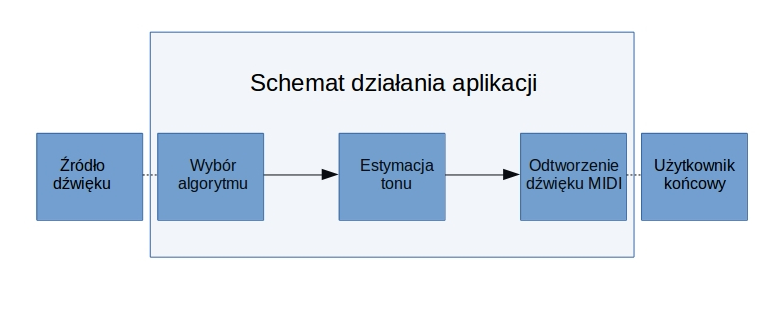
\includegraphics[width=0.5\linewidth]{rys/schematAplikacji}
  \caption{Schemat działania aplikacji.}
  \label{schemat}
\end{figure}


W jednym z pierwszych etapów przedstawionym na schemacie jest wybór odpowiedniego algorytmu. Algorytmy do wykrywania tonu prostego już istnieją i do realizacji tej pracy inżynierskiej nie ma potrzeby tworzenia nowych. Z istniejących rozwiązań, do realizacji zadania zostały wykorzystane algorytmy:

\begin{itemize}
\item[•]{YIN,}
\item[•]{MPM,}
\item[•]{Dynamic Wavelet,}
\item[•]{AMDF.}
\end{itemize}
 \section{{YIN}}
 YIN \cite{YIN} jest algorytmem do estymacji częstotliwości podstawowej mowy oraz dźwięków muzycznych, zawierającym kilka pożądanych cech, które zdecydowały o jego użyciu w aplikacji. W głównej mierze bazuje na metodzie autokorelacji z niewielkimi modyfikacjami pozwalającymi uniknąć błędów. YIN ma kilka parametrów, które nie wymagają precyzyjnego ustawienia. W przeciwieństwie do większości innych metod górny limit nie musi znajdować się w zakresie wyszukiwania $F_0$. Jego realizacja jest stosunkowo prosta i wystarczająco wydajna przy niewielkim opóźnieniu. Jedną z modyfikacji pozwalających uniknąć błędów jest wykonanie funkcji różnicowej. Na rysunku \ref{yin_mowa} został przedstawiony przykład sygnału uzyskanego z rejestracji mowy. Na rysunku \ref{yin_róznicowa} przedstawiony jest wynik użycia funkcji różnicowej.
 
  \begin{figure}[h!]
  \centering
  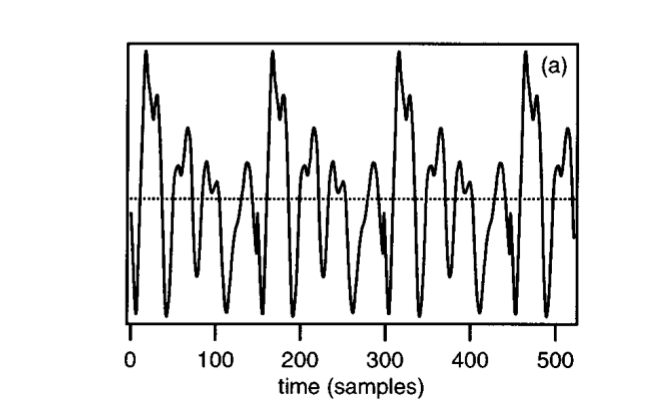
\includegraphics[width=0.7\linewidth]{rys/yin2}
  \caption{Przykładowy sygnał zarejestrowanej mowy \cite{YIN}.}
  \label{yin_mowa}
\end{figure}

  \begin{figure}[h!]
  \centering
  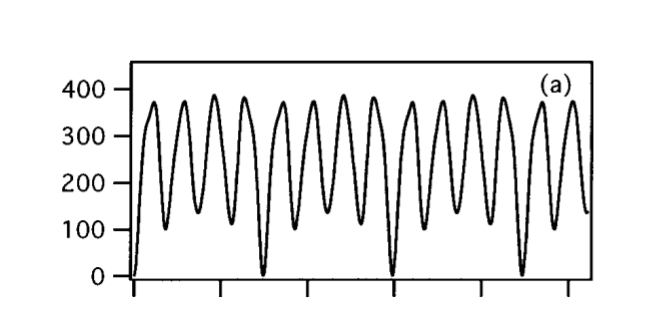
\includegraphics[width=0.7\linewidth]{rys/yin21}
  \caption{Sygnał mowy po użyciu funkcji różnicowej \cite{YIN}.}
  \label{yin_róznicowa}
\end{figure}

 \section{{MPM}}
 MPM \cite{harvey} (ang. McLeod Pitch Method) jest algorytmem również bazującym na metodzie autokorelacji. Może działać w czasie rzeczywistym ze standardowym próbkowaniem 44.1 kHz. Działa bez zastosowania filtra dolnoprzepustowego i może pracować z dźwiękiem o wysokiej harmonicznej jak np. dźwięk generowany przez skrzypce. Rejestrowane zmiany przez ten algorytm mają niezawodną dokładność 1 centa. MPM działa również dobrze bez przetwarzania końcowego poprawy wysokości dźwięku, co jest powszechnie stosowane w przypadku innych algorytmów.
 \section{{Dynamic Wavelet}}
 Dynamic Wavelet \cite{harvey} jest to algorytm, który do wyznaczania wysokości tonu używa tzw. falki. Wykorzystuje on STFT (ang. Short-time Fourier transform) oraz okna o stałej liczbie oscylacji. Długość okna określa się jako stałą liczbę okresów w tej częstotliwości.
 Dla algorytmu Dynamic Wavelat należy użyć metody CWT(ang. Continuous Wavelet Transform) danej wzorem:
\begin{equation}
\label{equation:1}
    c(a, b) = \int f(t) \Psi (at + b)dt
\end{equation}
Gdzie wartość  $c(a, b)$ jest współczynnikiem CWT  obliczonym poprzez splatanie sygnału $f(t)$ z falką, $\Psi$, skala $a$ o przesunięciu $b$ w czasie.
CWT często odnosi się do wektora wszystkich współczynników dla danej skali.
Podczas przetwarzania dużych sygnałów lub wielowymiarowych sygnałów, nadmiarowe dane sprawiają, że proces nie będzie możliwy do obliczenia. Wprowadzona została również Szybka transformacja falkowa (FWT)(ang. Fast Wavelet Transformation). FWT eliminuje problem nadmiarowości dzięki wykorzystaniu ortogonalności. Para funkcji jest ortogonalna, jeżeli ich iloczyn skalarny wynosi zero. Oznacza to, że każda informacja zakodowana przez pierwszą falkę, nie jest zakodowana przez drugą i odwrotnie. Zatem nie traci  się czasu na obliczanie nadmiarowych danych.
 \section{{AMDF}}
 AMDF \cite{AMDF} (ang. Average  Magnitude Difference Function) używa metody, która jest odmianą autokorelacji. Algorytm, zamiast korelować dane wejściowe przy różnych opóźnieniach (gdzie mnożenia i dodawania są tworzone dla każdej wartości) tworzy sygnał różnicowy pomiędzy dźwiękiem opóźnionym a oryginalnym i dla każdej wartości opóźnienia przyjmowana jest wartość bezwzględna. W przeciwieństwie do autokorelacji algorytm AMDF nie wymaga żadnych mnożeń, co jest pożądane we właściwościach dla aplikacji czasu rzeczywistego. Dla każdej wartości opóźnienia dokonuje się na oknie integrującym z $N$ próbek. Aby wygenerować cały zakres opóźnień, okno jest różnicowane krzyżowo z pełnym przedziałem analizy. Zaletą takiego rozwiązania są stałe opóźnienia. Wynika to z tego, że zawsze występuje pełne pokrywanie się danych pomiędzy dwoma segmentami różnicowania krzyżowego. AMDF może zostać użyty do rozpoznania wysokości tonu mowy. Jednak mowa zawiera bardzo bogate składowe harmoniczne. Minimalna $F_0$ wynosi około 80 Hz, a maksymalna 500 Hz. Większość jest w zakresie od 100 do 200 Hz. Więc sygnał może zawierać 30 do 40 składowych harmonicznych. Przy czym $F_0$ nie jest dominująca. Bogate składowe harmoniczne umożliwiają bardzo skomplikowane śledzenie dźwięku. Często zawierają błędy harmoniczne. Jednak nie jest konieczne dalsze przetwarzanie sygnału. Ponieważ zakres $F_0$ mieści się w zakresie 80 do 500 Hz. Składowe częstotliwości powyżej 500 Hz są bezużyteczne dla wykrywania tonu.
 Na rys. \ref{amdf1} został przedstawiony wykres śledzenia częstotliwości przez algorytm AMDF.  Dla porównania na rys. \ref{amdf2} został umieszczony wykres śledzenia częstotliwości z użyciem metody autokorelacji.
 
   \begin{figure}[h!]
  \centering
  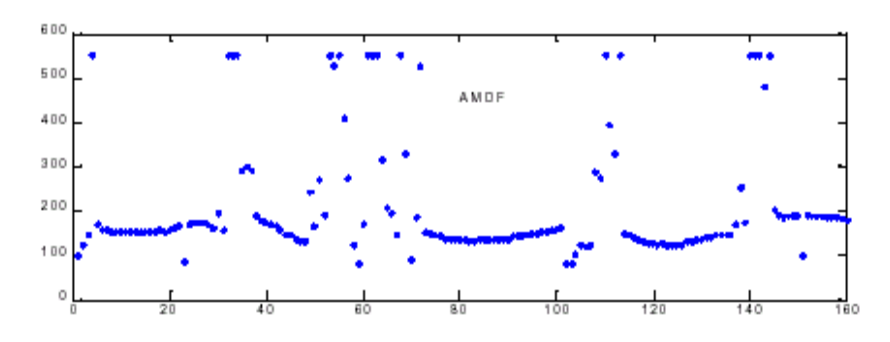
\includegraphics[width=0.7\linewidth]{rys/amdf1}
  \caption{Sygnał zarejestrowanej mowy \cite{AMDF}.}
  \label{amdf1}
\end{figure}

   \begin{figure}[h!]
  \centering
  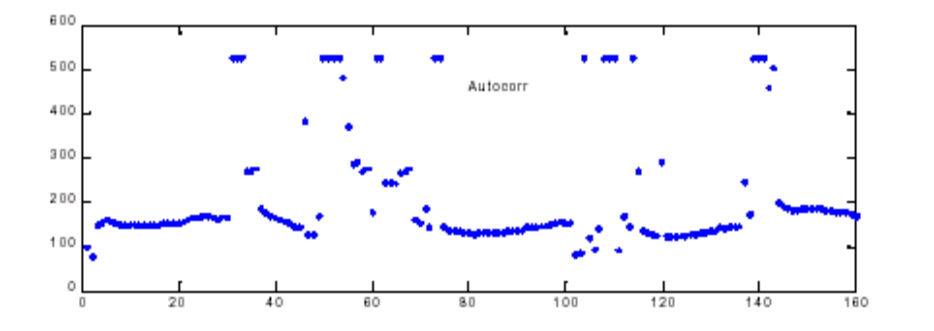
\includegraphics[width=0.7\linewidth]{rys/amdf2}
  \caption{Sygnał mowy po użyciu funkcji różnicowej \cite{AMDF}.}
  \label{amdf2}
\end{figure}

 \section{{Autokorelacja}}
Metoda autokorelacji wykorzystana w algorytmach YIN oraz MPM można obliczyć ze wzoru:
\begin{equation}
\label{equation:2}
   Rxx(n) = \sum_{m=0}^{M-1}{x(m)x(m+n)}
\end{equation}
Gdzie $Rxx$ jest dyskretną autokorelacją o opóźnieniu $l$, a $x(m)$ jest sygnałem dyskretnym. Metoda na wejściu przyjmuje sygnał okresowy. Po jej wykonaniu uzyskuje się wykres przedstawiający piki przy wielokrotności czasu. Metoda
  wyznaczania wysokości dźwięku określa jego wysokość na podstawie pozycji
  ($T_0$) dominującego pierwszego piku funkcji autokorelacji ($R_{xx}$).
  A jego częstotliwość określa zależność: $f_0=\frac{1}{T_0}$. Może pokazywać błędy, jeżeli dolne ograniczenie jest zbyt blisko zera, wtedy algorytm może błędnie wybrać szczyt. Również w przypadku ustawienia zbyt dużego ograniczenia algorytm może wybrać szczyt z kolejnego rzędu.

 \begin{figure}[h!]
  \centering
  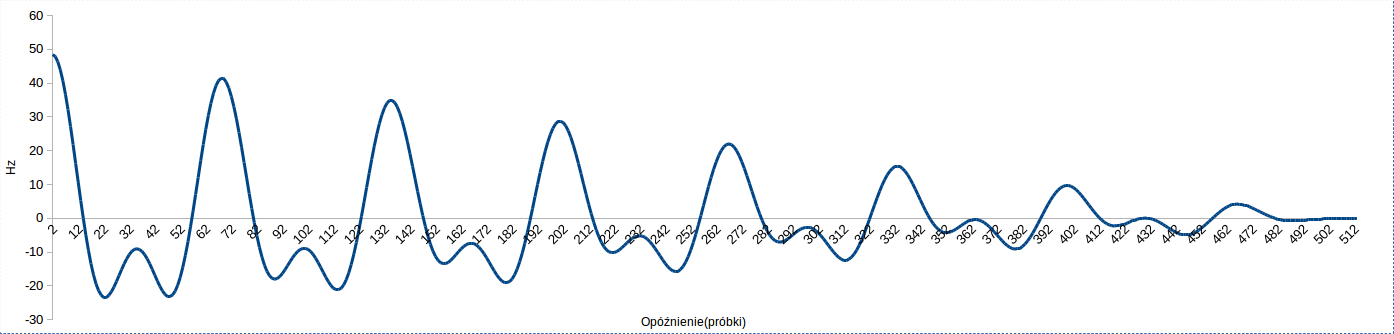
\includegraphics[width=0.7\linewidth]{rys/autocorelation}
  \caption{Przykładowy sygnał po użyciu metody autokorelacji}
  \label{autocorelation}
\end{figure}
Na rysunku 2.4 przedstawiony został wykres zawierający wartości poszczególnych próbek po użyciu wzoru na autokorelacje.


\section{{Przegląd istniejących aplikacji}}
Pierwszym z najbardziej popularnych programów nawiązujących do tematyki pracy jest program o nazwie „Jam Origin” przedstawiony na rysunku \ref{jamOr}. 


\begin{figure}[h!]
  \centering
  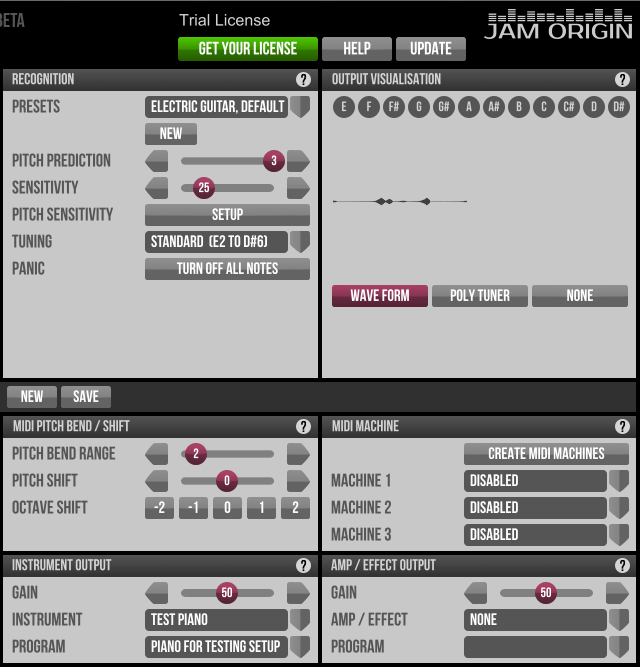
\includegraphics[width=0.5\linewidth]{rys/jamOrigin1}
  \caption{Zrzut ekranu z aplikacji Jam Origin. Źródło: www.jamorigin.com}
  \label{jamOr}
\end{figure}


Głównymi zaletami aplikacji są rozbudowane funkcje konfiguracji, jako że budowa instrumentów znacząco różni się ze względu na podział np.: smyczkowe, dęte. W większości przypadków można skonfigurować aplikacje pod daną kategorię, poczynając od instrumentów wydobywających pojedynczy dźwięk, aż po instrumenty wytwarzające kilka dźwięków jednocześnie. Najbardziej trafnym przykładem odnoszącym się do instrumentów wytwarzających kilka dźwięków jest gitara elektryczna. Aplikacja „Jam Origin” pozwala na jawne rozdzielenie kilku zagranych dźwięków lub wybieranie trybu mapowania tylko pojedynczego dźwięku. Ma to szczególne znaczenie przy dokładności i wierności odtwarzania wysokości tonów. Program ma też takie funkcje jak czułość przechwytywania dźwięku, co powoduje rzadsze pojawianie się błędów i daje możliwość dopasowania aktualnego poziomu wzmocnienia na wejściu do czułości przechwytywania.


Kolejnym wartym uwagi programem, zaliczającym się do aplikacji konwertującej dźwięk na  MIDI  jest przedstawiony na rysunku \ref{migic} „ Migic”. Zasada działania aplikacji jest podobna do poprzedniego przykładu, lecz główną różnicą pomiędzy tymi programami jest zbiór funkcji udostępniony użytkownikowi. Mianowicie „Migic” posiada wszystkie funkcje poprzednika oraz dodatkowo udostępnia pokaźną liczbę informacji.

\begin{figure}[h!]
  \centering
  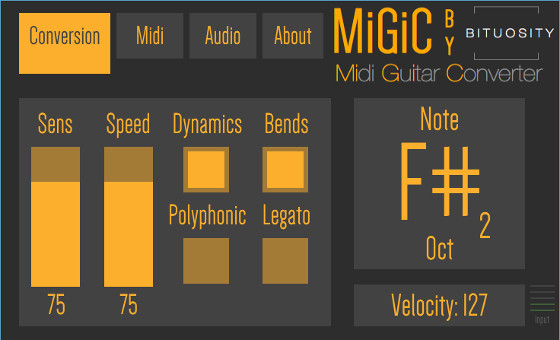
\includegraphics[width=0.5\linewidth]{rys/MIGIC1}
  \caption{Zrzut ekranu z aplikacji MiGiC. Źródło: migic.com}
  \label{migic}
\end{figure}

Do najważniejszych z nich zaliczą się: informacja o opóźnieniu pomiędzy zagranym dźwiękiem, a jego odpowiednikiem w interfejsie MIDI.
Również przydatną informacją jest wyświetlanie tonacji aktualnie granych dźwięków w formie graficznej. Ponadto program udostępnia różnego rodzaju efekty takie jak, pogłosy, echo, zmianę tonacji dźwięku w czasie rzeczywistym.
Przedstawione programy są jednymi z najbardziej popularnych programów komputerowych nawiązujących tematyką do tej pracy. Istotnym faktem jest to, iż na rynku istnieje jeszcze kilka rozwiązań konwersji dźwięku na MIDI. Jednakże są to rozwiązania rozbieżne z tematem pracy, ponieważ są w dużej mierze realizowane na poziomie sprzętowym z dedykowanymi programami na systemy wbudowane.


\section{{Standard MIDI}}

Standard MIDI \cite{MIDI} jest to format u standaryzowany w 1983 roku. Format ten nie zawiera bezpośredniego zapisu dźwięku. Zawiera szereg informacji, za pomocą których możemy uzyskać dźwięk na urządzeniu obsługującym ten format. Odgrywane sekwencje w postaci programowej można przyrównać do zapisu nutowego lub do pozytywek na taśmy perforowane. W formie sekwencji zapisywane są polecenia note on oraz note off. Każdemu z tych poleceń przypisane są informacje w postaci atrybutów tj.

\begin{itemize}
\item[•]{key velocity zawiera informacje o sile nacisku na konkretny klawisz syntezatora,}
\item[•]{wysokość tonu,}
\item[•]{modulacja dźwięku,}
\item[•]{clock jest to informacja na temat synchronizacji czasowej pomiędzy poszczególnymi dźwiękami.}
\end{itemize}

Za pomocą tych informacji urządzenie jest w stanie odtworzyć sekwencje poleceń.  MIDI jest dość starym standardem, jednak jego specyfikacja nie uległa zmianie, przez co zachowuje pełną kompatybilność ze wszystkimi urządzeniami obsługującymi ten standard. Aktualnie standard MIDI jest wykorzystywany do sterowania różnego rodzaju syntezatorami i samplerami, w tym także wirtualnymi. W przypadku tej pracy inżynierskiej wykorzystywany będzie syntezator wirtualny. 


Istotną kwestią w pracy z  MIDI jest opóźnienie. Występuje ono w komunikacji pomiędzy sekwencerem MIDI, czyli w tym wypadku pierwszej części aplikacji, która odpowiedzialna jest znalezienie wysokości tonu i przesłanie go komunikatem MIDI, a urządzeniem odbiorczym, w tym przypadku druga część aplikacji odpowiadająca za odtwarzanie dźwięku. Na opóźnienie składa się również czas, jaki potrzebny jest na przetworzenie komunikatu w urządzeniu odbiorczym.


W standardzie MIDI występują kanały. Każdy kanał może zawierać inną treść podczas transmisji. Przykładowo na każdym kanale można przesyłać różne identyfikatory instrumentów oraz odpowiednie dla nich sekwencje pojedynczych nut lub ich zbiorów. Ważną rzeczą w tym założeniu jest fakt, iż tak naprawdę na stacji odbiorczej do każdego kanału dopasowuje się konkretny instrument. Odtworzony dźwięk będzie oczywiście brzmiał inaczej jeżeli np. na kanale zawierającym partię perkusyjne ustawiony zostanie np. fortepian. Podczas komunikacji pomiędzy różnymi urządzeniami należy zatem za każdym razem sprawdzić, czy ustawienia kanałów są zgodne z pierwowzorem. Problemy te związane były między innymi z różnicami wynikającymi z brakiem współpracy producentów. Jest to problematyczne jednak aktualnie w większości przypadków urządzenia  oraz programy wykorzystujące MIDI używają standardu General MIDI.


Standard ten został wprowadzony w 1991 roku. Jego założenia miały na celu usystematyzowanie dostępnych instrumentów, ponieważ kontrolowanie ustawień konkretnych instrumentów na danych kanałach zdecydowanie zaburzało łatwość komunikacji. Został wprowadzony bank 128 brzmień. General MIDI obligował producentów i twórców oprogramowania do zachowania kompatybilności dźwięku instrumentów czy efektów. Dla przykładu na pierwszych sześciu pozycjach znajdują się wariacje dźwięku pianina, następnie organ, gitar oraz instrumentów basowych. Oprócz u standaryzowania instrumentów zostały także postawione wytyczne co do wysokości tonów dla instrumentów perkusyjnych. Obsługa zwiększonej liczby instrumentów nadal pozostaje kompatybilna ze standardem zapisu SMF.


SMF (ang. Standard MIDI Files) - Standard jednolitego zapisu informacji dla sekwencerów. Pomimo iż każda firma do swojego sprzętu oraz aplikacji bazujących na MIDI, używa swojego specjalistycznego sposobu zapisu danych, większość urządzeń oraz aplikacji obsługuje standard SMF. Sytuacja ma się inaczej w przypadku dodatkowych informacji dostępnych tylko i wyłącznie dla konkretnych modeli urządzeń lub serii produktów, w skład którego również wchodzi oprogramowanie. Informacje te zostają utracone. Nie wpływa to na odtwarzany dźwięk na urządzeniu końcowym.
Zostały utworzone trzy wersje formatu SMF, oznaczone kolejno 0, 1, 2 . W chwili pisania pracy standard jest nadal w użytku i służy do wymiany informacji pomiędzy urządzeniami i  aplikacjami obsługującymi format MIDI. W użytku pozostaje wersja 0 oraz 2. Głównymi różnicami pomiędzy tymi dwoma wydaniami standardu SMF jest sposób zapisu. Dla formatu oznaczonego numerem 0 zapis odbywa się na jednej ścieżce. Jest to dopuszczalny sposób ze względu na to, iż każde zdarzenie MIDI ma w sobie zawartą informację o numerze kanału. Po załadowaniu pliku zapisanego w formacie SMF w wersji 0, urządzenie odbiorcze może bez problemu rozdzielić pojedynczą ścieżkę na wiele ścieżek. Jest to pewna niedogodność, która nie występuje w przypadku wersji 1. W tym wariancie plik zawiera informacje MIDI w formacie wielościeżkowym. Zaletą tego jest niewątpliwie to, że załadowany plik jest bezpośrednio gotowy do użycia lub edycji.


Na rysunku \ref{midiWizual} przykładowa wizualizacja zapisu formatu MIDI w programie FL Studio.

\begin{figure}[h!]
  \centering
  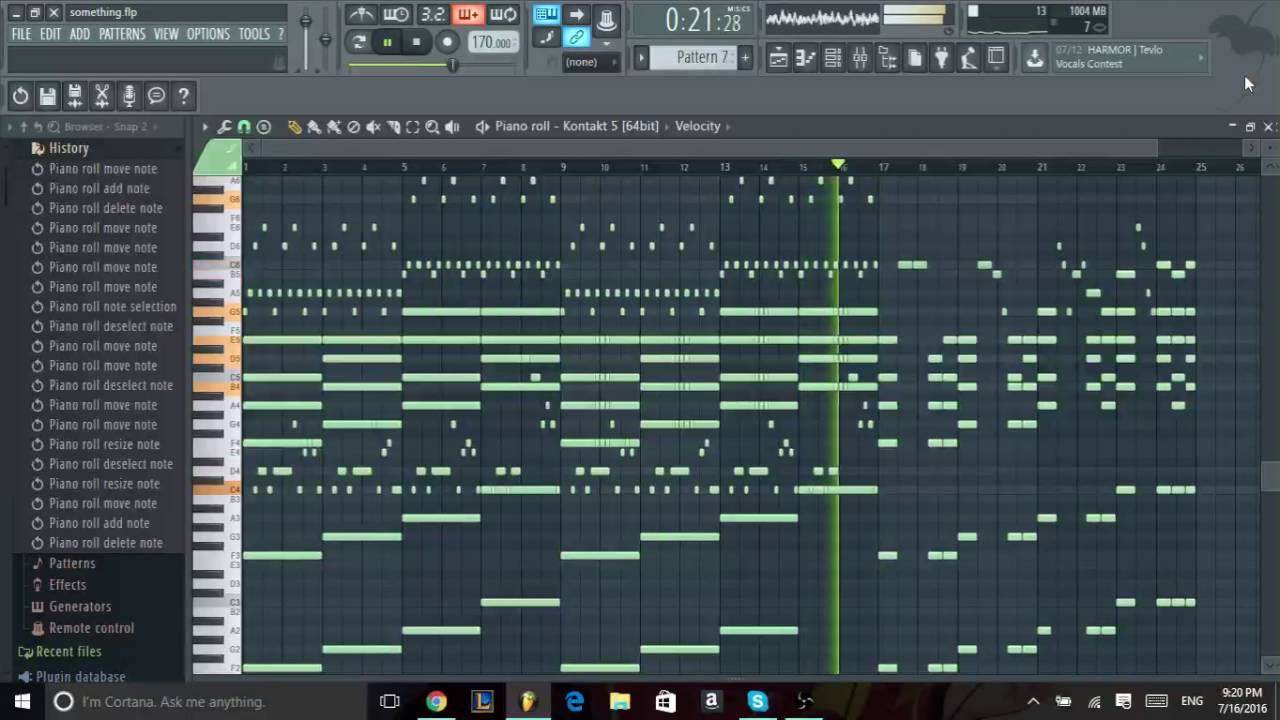
\includegraphics[width=0.5\linewidth]{rys/fl1}
  \caption{Zrzut ekranu z aplikacji FL Studio. Źródło: www.image-line.com/flstudio}
  \label{midiWizual}
\end{figure}


Synchronizacja MIDI jest potrzebna, aby przeprowadzić poprawną komunikację pomiędzy urządzeniami obsługującymi interfejs MIDI. Jest to jeden z fundamentalnych aspektów współpracy urządzeń oraz aplikacji. Jednym ze sposobów synchronizacji jest MIDI Sync (MIDI Clock). W tym rodzaju synchronizacji brane są pod uwagę następujące komunikaty:


\begin{itemize}
\item[•]{Start, komunikat ten zawiera informacje dla urządzenia odbiorczego o rozpoczęciu odtwarzania.}
\item[•]{Stop, komunikat ten zawiera informacje dla urządzenia odbiorczego o zatrzymaniu odtwarzania.}
\item[•]{Continue, komunikat ten zawiera informacje dla urządzenia odbiorczego o odtwarzania od wskazanego miejsca.}
\item[•]{Song Position Pointer, jest to komunikat nakazujący urządzeniu podrzędnemu zmianę w odtwarzaniu do określonego miejsca w utworze.}
\end{itemize}

Opis procesu synchronizacji wygląda następująco. Urządzenie wysyłające przekazuje informacje do urządzenia odbiorczego, w której zawarty jest komunikat zegarowy pracujący z częstotliwością 24 impulsy na ćwierć nutę. Oczywiście wynika z tego faktu zależności całego procesu od nadanego w utworze tempa. W przypadku gdy główny sekwencer zmieni tempo, zaczyna wysyłać większą liczbę impulsów na sekundę. Powoduje to zmianę tempa w urządzeniu odbiorczym.


Istnieje także inna metoda synchronizacji (ang. MIDI Time Code). Swoje główne zastosowanie znalazła dla obsługi przypadków, w których występuje potrzeba synchronizacji dźwięku oraz obrazu.  W tym typie synchronizacji należy odnieść się do czasu rzeczywistego wyrażonego w jednostkach: godzinach, minutach, sekundach. Jest to typ synchronizacji SMPTE, który nagrywany jest na osobnych ścieżkach rejestratora. Wykorzystuje generator kodu czasowego. Dzięki zastosowaniu oznaczeń czasowych urządzenie odbiorcze jest w stanie zsynchronizować się w każdym momencie trwania utworu. Aby było można w pełni wykorzystać oznaczenia czasowe, należy wyposażyć urządzenia w konwertery (sprzętowe lub programowe), które potrafią przetwarzać kod SMPTE na MIDI Time Code (MTC). Jest to kod spełniający funkcję analogiczną do powyższego, z tą różnicą, że nie pracuje w oparciu o sygnał audio. Kod MTC wykorzystuje specjalne komunikaty MIDI. Urządzenie odbiorcze po otrzymaniu komunikatu, na którym swoją pracę opiera MTC, ma za zadanie zamianę tych informacji na takty, bity oraz impulsy zegara są adekwatne do odpowiadających im jednostek czasu rzeczywistego. Powyższe rozwiązania nie są jednak na tyle dokładne, aby były wykorzystywane osobno do profesjonalnych zastosowań. Do takich zastosowań wykorzystywany jest Word Clock. Jest to sygnał zegarowy, który jest w pełni kompatybilny z pojedynczym impulsem próbkującym. 



\section{{Środowiska programistyczne}}

Aktualnie istnieje wiele rozbudowanych zintegrowanych środowisk programistycznych. Jednakże dla każdego istnieje uzasadnione przeznaczenie.

\begin{itemize}
\item[•]{Xcode,}
\item[•]{Eclipse,}
\item[•]{Netbeans.}
\end{itemize}


Xcode \cite{Xcode} jest zintegrowanym środowiskiem programistycznym stworzonym przez firmę Apple Inc. Wykorzystywany jest do tworzenia oprogramowania różnego rodzaju na systemy operacyjne OS X. Posiada rozbudowane funkcje: edycji plików, nawigacji po projekcie oraz  debugowania wszystkich typów projektów programistycznych OS X, włączając w to aplikacje, narzędzia, schematy, biblioteki, pakiety pluginowe, rozszerzenia jądra i sterowniki urządzeń. Xcode współpracuje także z systemem kontroli wersji Git poprzez zintegrowane funkcjonalności i specjalnie przeznaczone do tego interfejsy dostępne dla programisty. Wszystkie potrzebne komendy zostały zaopatrzone w łatwy w obsłudze interfejs graficzny, co znacznie upraszcza zarządzanie projektem.


Kolejne IDE, które cieszy się dużą popularnością to NetBeans \cite{netbeans}. Jest to środowisko udostępnione bezpłatnie na większość dostępnych systemów operacyjnych. Środowisko to posiada szereg zalet i można uznać je za jedno z najlepszych środowisk programistycznych. Jest oficjalnym środowiskiem programistycznym dla Javy w wersji 8. NetBeans jako darmowe IDE jest przygotowane w kilku wersjach, przeznaczonych do różnych języków programowania. Edytor wspiera wiele składni języków takich jak:  Java, C/C++, XML, HTML, PHP, GROOVY, Javadoc i JavaScript. Edytor tego środowiska jest bardzo elastyczny i pozwala na rozszerzenie wsparcia dla większej liczby języków. Posiada również mechanizm uzupełniania składni oraz całych konstrukcji takich jak: wyrażenie warunkowe, pętle, instrukcje warunkowe. W przypadku pracy z dużym projektem  twórcy IDE udostępnili efektywne i proste w obsłudze narzędzia do zarządzania.


Wybrane środowisko do tworzenia aplikacji to Eclipse \cite{eclipse}. Jest to platforma programistyczna istniejąca od 2004 r. oparta na języku Java. Głównym powodem wyboru tego IDE, jest prostota użytkowania. Kolejnym argumentem, który przemawia za wyborem tego środowiska, jest między innymi fakt, iż jest to najbardziej rozbudowane środowisko. Środowisko to jest przygotowane do pracy z kilkoma językami programowania w zależności od wersji. Jest aktualnie najczęściej wybieraną platformą do tworzenia aplikacji w języku Java. Całość środowiska jest uzupełniona poprzez dołączane plug-iny.  Ten sposób tworzenia środowiska umożliwia odpowiednie dopasowanie go do potrzeb użytkownika. Użytkownik ma również dostęp do bazy pluginów.


\begin{itemize}
\item[•]{Standardowa wyszukiwarka plików znajdujących się w projekcie.}
\item[•]{Przeszukiwanie plików pod kątem zdeklarowanego tekstu, można używać tu standardu wyrażeń regularnych oraz ograniczyć przeszukiwanie do konkretnych katalogów.}
\item[•]{Lista klas potomnych dla konkretnej klasy oraz lista interfejsów, które są zaimplementowane w klasie.}
\end{itemize}


Na rysunku \ref{eclipse} został przedstawiony zrzut ekranu wybranego środowiska programistycznego Eclipse.


\begin{figure}[h!]
  \centering
  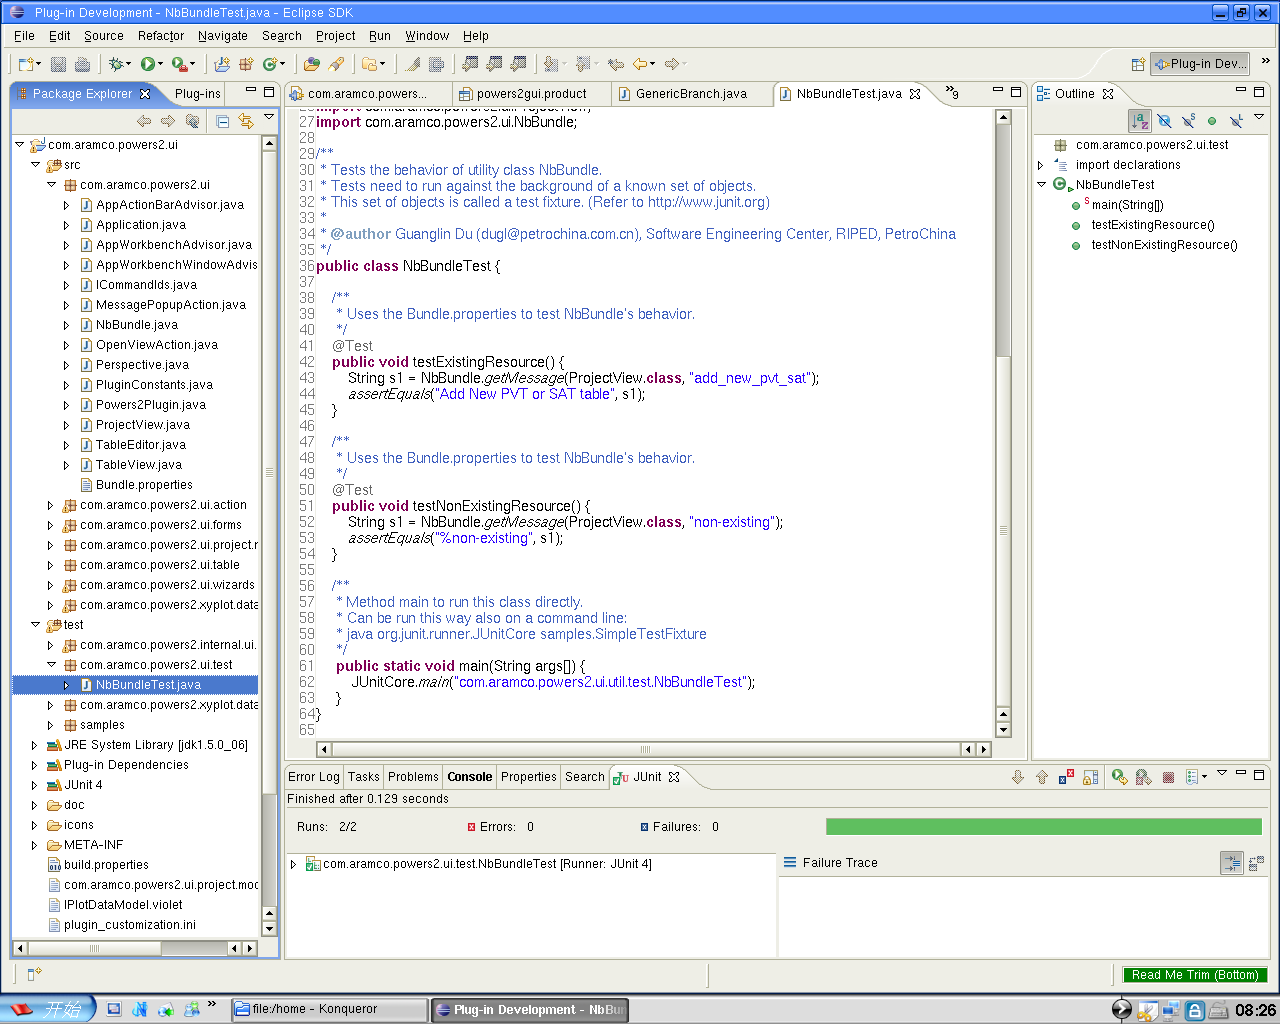
\includegraphics[width=0.5\linewidth]{rys/eclipse1}
  \caption{Środowisko programistyczne Eclipse.}
  \label{eclipse}
\end{figure}

\section{{Języki programowania i biblioteki}}

Do zrealizowania aplikacji użyty zostanie język Java. Jest to jeden z najbardziej popularnych języków. 
Java \cite{horstmann} jest językiem, który z założenia miał być prosty, oznacza to, że struktura języka nie jest skomplikowana. Dopatrując się podobieństw, można zauważyć, iż składnia języka jest zbliżona ze składnią C++.  Język ten jest w pełni obiektowy, co w dużej mierze ułatwia projektowanie bardziej złożonych systemów. Twórcy języka postawili również na niezawodność, jednym z argumentów za tym przemawiających jest fakt, iż model wskaźnikowy w tym języku jest zaprojektowany w przemyślany sposób. Nie ma tutaj możliwości nadpisania pamięci i zniszczenia danych, które się w niej znajdują. Mechanizmy abstrakcji zastosowane w tym języku pozwalają na znacznie lepszą i efektywniejszą organizację samego kodu źródłowego, jak również podział logiczny. 


Język ten ma znaczną przewagę na innymi językami programowania,  ze względu na zastosowanie obiektowości oraz ze względu na wiele nowych przydatnych funkcji dodanych w kolejnych odsłonach języka. Z każdą wersją dodawane są nowe funkcjonalności, które w znacznym stopniu ułatwiają pracę programisty. Przestarzałe funkcjonalności są oznaczane jako przestarzałe. Na ich miejsce pojawiają się nowe, co świadczy o tym, iż język ten jest ciągle rozwijany \cite{horstmann}. 


Java dysponuje też pokaźną liczbą gotowych bibliotek. Biblioteki te w większości przypadków wyręczają programistów. Gotowe rozwiązania znacznie usprawniają i przyspieszają pracę. Umożliwia to zaoszczędzenie dużej ilości czasu poprzez udostępnianie, chociażby gotowych rozwiązań z zakresu struktur danych.


Główną zaletą popularności języka jest to, iż istnieje dostęp do dużej liczby kodów źródłowych zawierających gotowe rozwiązania lub opis wraz z rozwiązaniami wielu ważnych problemów pojawiających się stale, przy projektowaniu różnorodnych aplikacji.


Ważnym aspektem w języku Java \cite{horstmann2} jest fakt, że programy napisane w tym języku  po kompilacji do plików w formacie obiektowym są uruchamiane na maszynie wirtualnej. Możemy zatem uruchamiać aplikacje na wszystkich urządzeniach, które obsługują i mają zainstalowaną Javę. Dzieje się tak dlatego, iż kompilator tworzy kod bajtowy niezależny od żadnego procesora. Kod tak wygenerowany jest tworzony w ten sposób, aby jak najszybciej można było go przetłumaczyć na kod maszynowy procesora.


Istotną kwestią przy utrzymywaniu dobrego stylu programowania jest utrzymywanie przejrzystej dokumentacji. Zarządzanie dokumentacją odbywa się przy pomocy narzędzia JavaDoc. Za pomocą znaczników, które umieszczane są w kodzie źródłowym, Java jest w stanie wygenerować przejrzystą dokumentację w języku HTML. Używanie znaczników nieznacznie różni się od umieszczania komentarzy. Zostało to rozróżnione, ponieważ nie wszystkie komentarze powinny znajdować się w ogólnej dokumentacji. Blok zdefiniowany na potrzeby Javadoc jest ignorowany przez kompilator. Umieszczenie bloku przed deklaracją klasy lub metody stanowi jej opis. Do dyspozycji zostały oddane również znaczniki umożliwiające opis parametrów poszczególnych metod. 


Zdecydowanie się na konkretny język programowania niesie za sobą decyzje o konkretnych bibliotekach, z którymi praca jest znacznie szybsza, ponieważ zawierają one gotowe rozwiązania. Użyte w projekcje biblioteki to:


\begin{itemize}
\item[•]{jfreechart-1.0.19 jest to bardzo użyteczne narzędzie do tworzenia różnego rodzaju wykresów. W aplikacji główne zastosowanie biblioteka ta znalazła przy generowanie wykresu z pliku dźwiękowego w formacie Wav oraz przy generowaniu wykresu dźwięku w czasie rzeczywistym.}
\item[•]{jMusic1.6.5 jest to biblioteka która, znalazła zastosowanie w drugiej części aplikacji, w której w dużej mierze bazuje się na wykorzystaniu protokołu MIDI. Jej konstrukcja oraz przemyślana funkcjonalność pozwalają na tworzenie logicznych układów nut w protokole MIDI. Dużym ułatwieniem jest także wbudowany konwerter zamieniający podaną wartość w Hercach na odpowiadającą jej nutę.}
\item[•]{TarsosDSP jest to biblioteka zawierająca szeroką gamę zastosowań dotyczących przetwarzania dźwięku.}
\end{itemize}
Realizacja projektu w języku Java pomija problemy związane z obsługą interfejsów dźwiękowych różniących się od siebie w zależności od systemu operacyjnego. Jest to duże ułatwienie, ponieważ każdy system korzysta ze swoich interfejsów takich jak ALSA, JACK oraz OSS w przypadku Linuksa. Wsparcie dla DirectSound and ASIO w przypadku Windowsa oraz SGI w przypadku Macintosha.
\chapter{{Implementacja programowa systemu}}
\label{chapter:implementacja}
\thispagestyle{empty}

W niniejszym rozdziale pokazane zostały etapy budowania aplikacji. Poszczególne części rozdziału zawierają kolejno diagramy, opis budowy aplikacji oraz zrzuty ekrany gotowej aplikacji z podziałem na funkcjonalności.

\section{{Diagram klas}}

\begin{figure}[h!]
  \centering
  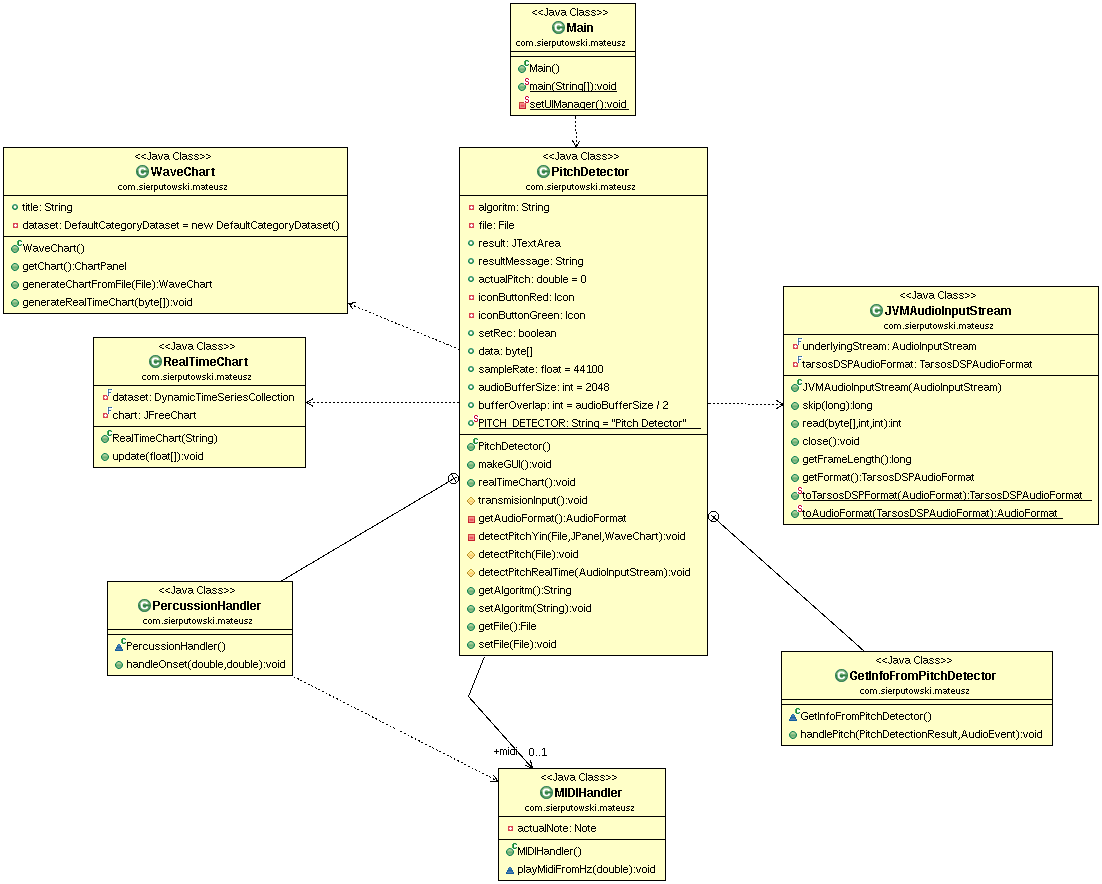
\includegraphics[width=1\linewidth]{rys/diagram1}
  \caption{Diagram klas.}
  \label{fig:schemat}
\end{figure}

Powyższy diagram przedstawia klasy użyte w tej pracy inżynierskiej. Główną klasą aplikacji jest klasa PitchDetector. Nazwa tej klasy odzwierciedla również nazwę aplikacji. Jest to główna klasa zawierająca interface graficzny użytkownika. Zawiera również obiekty obsługujące większość funkcjonalności aplikacji. Zawiera również niezbędne do poprawnego działania aplikacji ustawienia domyślne. 


Kolejną klasą zawartą w diagramie jest klasa WaveChart. Klasa ta jest odpowiedzialna za generowanie wykresów. Jest ograniczona jedynie do tworzenia wykresów na podstawie plików wczytanych z dysku. Aby rozszerzyć funkcjonalność, została również stworzona klasa odpowiedzialna za generowanie wykresów w czasie rzeczywistym z przekazywanego strumienia danych o nazwie RealTimeChart. Do obsługi strumieni danych oprócz standardowych bibliotek Javy została wykorzystana klasa JVMAudioInputStream. W celu realizacji jednego z dwóch głównych celów aplikacji zostały stworzone dwie klasy, kolejno GetInfoFromPitchDetector oraz PercussionHandler. Pierwsza z nich jest odpowiedzialna za wykrywanie tonów, druga zaś wykrywa rozpoczęcie trwania tonu w czasie. Aby zrealizować drugi cel aplikacji, użyta została klasa MIDIHandler, która zawiera obsługę protokołu MIDI.


\section{{Opis działania aplikacji}}

W tym rozdziale zostanie omówione działanie aplikacji. Sposób poruszania się po niej oraz obsługi.


Na rysunku zamieszczono zrzuty ekranu ukończonej aplikacji.

\begin{figure}[h!]
  \centering
  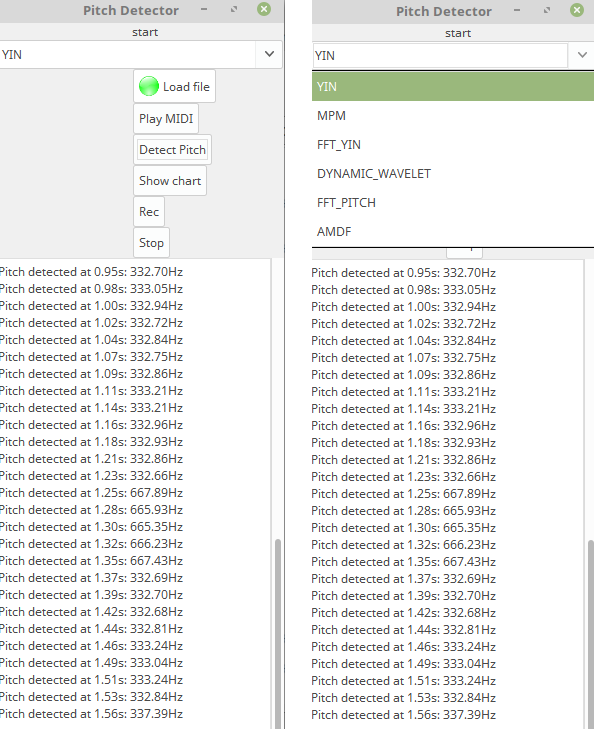
\includegraphics[width=0.5\linewidth]{rys/zrzut1}
  \caption{Zrzut ekranu aplikacjii.}
  \label{fig:schemat}
\end{figure}


Na zrzucie ekranu został przedstawiony interfejs graficzny użytkownika. Do wykonania GUI został wykorzystany pakiet Swing. W górnej części aplikacji znajdują się przyciski funkcjonalne, poniżej został wykorzystany komponent Text Area, który służy do wyświetlania informacji generowanych przez program. Został przedstawiony sposób wyboru algorytmu, który ma posłużyć do wykrywania tonu. Wykorzystany został również mechanizm obsługujący ładowanie plików z dysku.
\chapter{Badania eksperymentalne}
\label{chapter:rezultaty}

W tym rozdziale zostaną przedstawione wyniki badań skuteczności działania aplikacji oraz sposoby ich realizacji. Badania zostaną przeprowadzone w warunkach domowych.

\section{Opis badania}

Badanie ma na celu sprawdzenie skuteczności aplikacji poprzez wykrywanie tonu prostego ze źródła dźwięku znajdującego się w różniej odległości od mikrofonu. Jako generator dźwięku została użyta gitara akustyczna. Badanie zostało podzielone na 3 etapy. W pierwszym etapie zostanie wykorzystany przetwornik elektromagnetyczny podłączony do komputera, na którym uruchomiona jest aplikacja. Połączenie to zrealizowano za pomocą kabla gitarowego. Przewód zakończony jest wtykiem mono jack 6,3 mm. Na gitarze został odgrany jeden dźwięk o częstotliwości 440 Hz. Głośność urządzenia wejściowego, czyli mikrofonu podłączonego do komputera ustawiona jest na 40 db. W tym etapie odległość źródła dźwięku nie będzie miała znaczenia. Wyniki zostały przedstawione za pomocą wykresu słupkowego, gdzie oś X wyrażona jest w centymetrach. Odległość mikrofonu od źródła dźwięku została zwiększana co 40 cm. Oś Y wyrażona jest w  Hz i stanowić będzie średnią arytmetyczną 30 pierwszych pomiarów wysokości tonu prostego w czasie 0.5 sekundy. 

\section{Rezultaty badań}

Etap pierwszy przedstawia wyniki podłączenia przetwornika elektromagnetycznego zamontowanego w gitarze, z komputerem, na którym uruchomiona została aplikacja. Wyniki zostały przedstawione na rysunku \ref{kabel}.


\begin{figure}[h!]
  \centering
  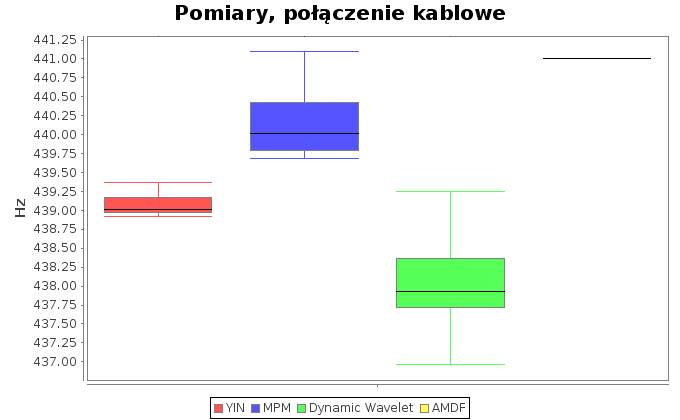
\includegraphics[width=0.9\linewidth]{rys/BoxPlots/kabel}
  \caption{Wykres przedstawiający wyniki połączenia kablowego.}
  \label{kabel}
\end{figure}





Algorytm AMDF we wszystkich pomiarach wskazywał dokładnie 441 Hz, więc te wyniki nie wymagają przedstawienia graficznego. Jak widać na rys \ref{yinwb} najmniejsza rozbieżność wartości została zanotowana przy użyciu metody YIN. Natomiast przy użyciu metody Dynamic Wavelet rozbieżność była największa. W przypadku algorytmu MPM mediana wartości osiągnęła częstotliwość 440 Hz. Była to częstotliwość odgrywana na instrumencie.
 
Kolejnym etapem jest wykonywanie pomiarów z zadanej odległości.


\begin{figure}[h!]
  \centering
  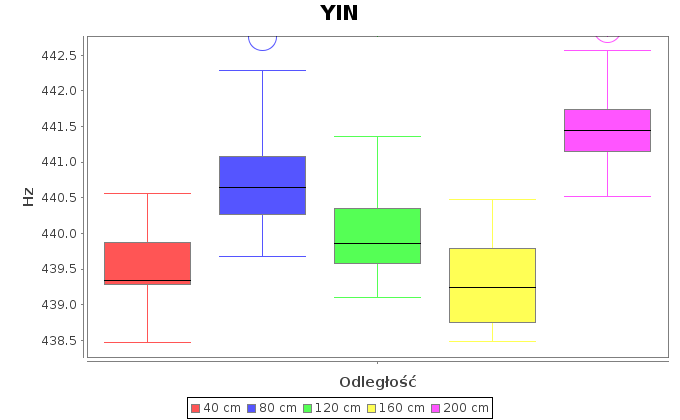
\includegraphics[width=0.9\linewidth]{rys/BoxPlots/YIN_mic_wb}
  \caption{Wykres przedstawiający wyniki przy użyciu algorytmu YIN oraz zastosowaniu mikrofonu wbudowanego.}
  \label{yinwb}
\end{figure}


Podczas tego etapu dodatkowym czynnikiem wpływającym na wyniki badań jest odległość, która została podana w opisie badania. Wykorzystany algorytm do przeprowadzenia tego pomiaru to YIN. Jest to pierwszy z czterech wybranych algorytmów. Wybór tego algorytmu został podyktowany przez chęć wykorzystania metody autokorelacji, której używa algorytm YIN. Jako urządzenie wejściowe został użyty standardowy wbudowany mikrofon. Jak można odczytać z wykresu na rys. \ref{mpmwb} wartości są zróżnicowane, lecz ich amplituda nie jest większa niż 2 Hz od częstotliwości 440 Hz. Jednak nie są one tak dokładne, jak w przypadku połączenia kablowego. Zbiór, z którego wyliczona mediana zwraca 440 Hz to zbiór, który powstał poprzez pomiar z odległości 120 cm.


\begin{figure}[h!]
  \centering
  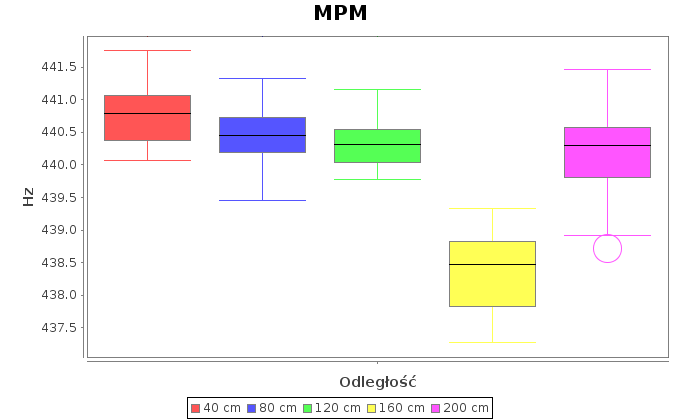
\includegraphics[width=0.9\linewidth]{rys/BoxPlots/MPM_mic_wb}
  \caption{Wykres przedstawiający wyniki przy użyciu algorytmu MPM oraz zastosowaniu mikrofonu wbudowanego.}
  \label{mpmwb}
\end{figure}


W tym wypadku do wykonania pomiarów został użyty algorytm MPM. Jak w poprzednim przypadku został również użyty standardowy wbudowany mikrofon. Jak można odczytać z wykresu na rys. \ref{dynamicwb} wartości z teoretycznie najdokładniejszego pomiaru, czyli 40 cm znajdują się w przedziale od 440.4 Hz do 441 Hz. Mediany kolejnych pomiarów są do siebie zbliżone. Wyjątek stanowi wynik pomiaru z odległości 160 cm. Znacznie odbiega od reszty. Strój instrumentu nie mógł ulec zmianie co potwierdza kolejny pomiar z większej odległości  w tym przypadku mógł zadziałać negatywnie na poprawność wyników czynnik, jakim są zakłócenia występujące podczas pomiaru.


\begin{figure}[h!]
  \centering
  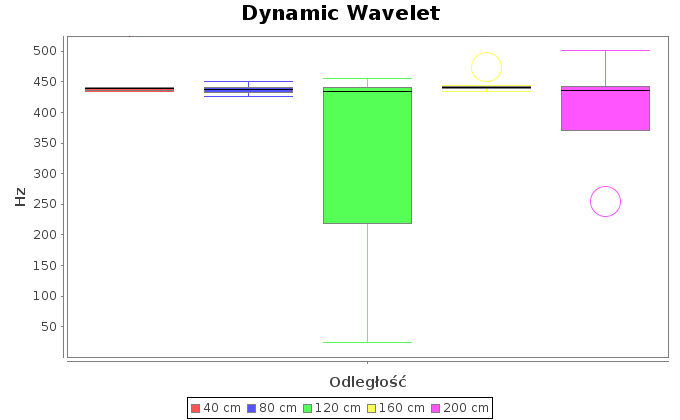
\includegraphics[width=0.9\linewidth]{rys/BoxPlots/Dynamic_mic_wb}
  \caption{Wykres przedstawiający wyniki przy użyciu algorytmu Dynamic Wavelet oraz zastosowaniu mikrofonu wbudowanego.}
  \label{dynamicwb}
\end{figure}

Kolejny pomiar dotyczy wykorzystania algorytmu Dynamic Wavelet. W tym przypadku również jak w dwóch poprzednich został użyty ten sam mikrofon jako urządzenie wejściowe. Jak można odczytać z wykresu na rys. \ref{yinz} rozbieżność wyników pomiaru z odległości 120 cm spowodowała przeskalowanie wykresu. W tym wypadku również dużą rozbieżnością charakteryzuje się pomiar z odległości 200 cm. Reszta pomiarów oscyluje wokół częstotliwości 440 Hz.


\begin{figure}[h!]
  \centering
  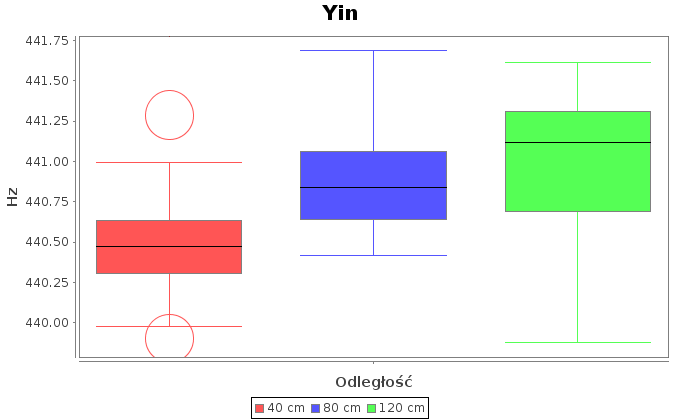
\includegraphics[width=0.9\linewidth]{rys/BoxPlots/YIN_mic_zew}
  \caption{Wykres przedstawiający wyniki przy użyciu algorytmu YIN oraz zastosowaniu mikrofonu zewnętrznego.}
  \label{yinz}
\end{figure}



Podczas kolejnego zbioru pomiarów został użyty algorytm YIN, jednakże z mikrofonem zewnętrznym. Przedstawiony wykres na rys. \ref{mpmz} zawiera jedynie 3 odległości z powodu tego, iż nie sprawdził się na większe odległości i kolejne próby jej zwiększania dawały wynik równy zero. Wszystkie pomiary mieszczą się w granicach od 440 Hz do 441 Hz, co można uznać za satysfakcjonujący wynik.


\begin{figure}[h!]
  \centering
  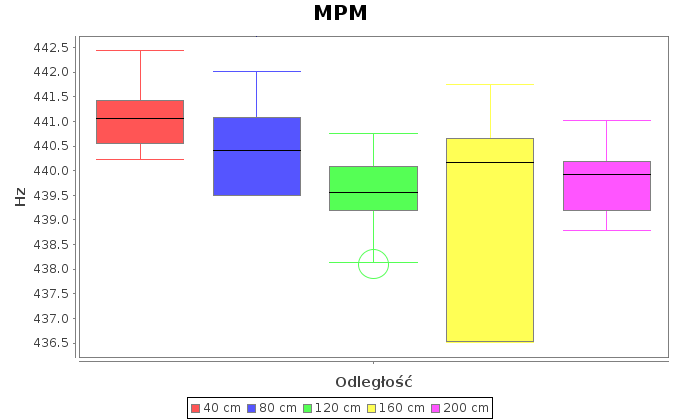
\includegraphics[width=0.9\linewidth]{rys/BoxPlots/MPM_mic_zew}
  \caption{Wykres przedstawiający wyniki przy użyciu algorytmu MPM oraz zastosowaniu mikrofonu zewnętrznego.}
  \label{mpmz}
\end{figure}


W tym przypadku został ponownie zastosowany algorytm MPM jednak dla uzyskania tych pomiarów użyto mikrofonu zewnętrznego. Algorytm zdecydowanie lepiej poradził sobie z odległością niż jego poprzednik. Jedyny pomiar z dużą rozbieżnością danych to pomiar z 160 cm. Zostało to przedstawione na wykresie na rys. \ref{dynamiz} Prawdopodobnie wynikał on z zakłóceń występujących podczas dokonywania pomiaru. Do zakłóceń możemy zaliczyć: szum generowany przez wentylator komputera. Mediany pomiarów ze wszystkich odległości oscylują wokół częstotliwości 440 Hz, czyli oczekiwanej.



\begin{figure}[h!]
  \centering
  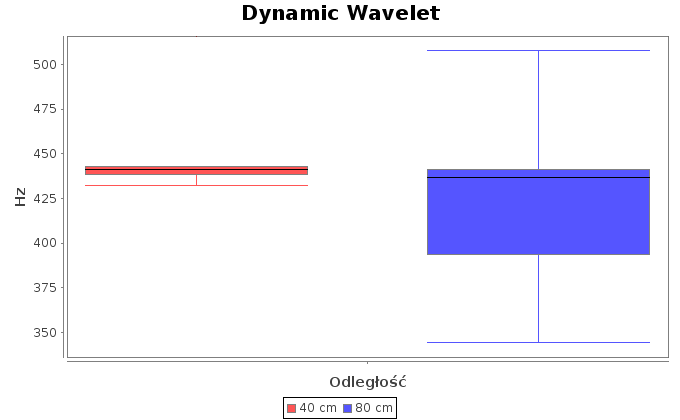
\includegraphics[width=0.9\linewidth]{rys/BoxPlots/Dynamic_mic_zew}
  \caption{Wykres przedstawiający wyniki przy użyciu algorytmu Dynamic Wavelet oraz zastosowaniu mikrofonu zewnętrznego.}
  \label{dynamiz}
\end{figure}

Ostatnim z przedstawionych wykresów jest wykres na rys 4.7, który obrazuje pomiary wykonane przy użyciu algorytmu Dynamic Wavelet oraz mikrofonu zewnętrznego. Na tym wykresie zostały przedstawione tylko dwa zbiory pomiarów. Z odległości 40 oraz 80 cm. Przy większej odległości wynik wynosił 0. Przy pierwszej odległości wynoszącej 40 cm. Mediana, jak i wszystkie pomiary z wyjątkiem wartości skrajnej są w przedziale od 440 Hz do 441 Hz. Taki wynik jest zadowalający. Przypadku tej konfiguracji tj. algorytmu Dynamic Wavelet oraz mikrofonu zewnętrznego można zauważyć coraz większą rozbieżność wyników.


Na koniec warto wspomnieć o algorytmie AMDF. Nie zostały zamieszczone wykresy oraz tabele z dokładnymi pomiarami przedstawiające wyniki tego algorytmu, ponieważ we wszystkich pomiarach rezultat wynosił 441 Hz.

Podsumowując przeprowadzone badania, można wywnioskować, iż działanie aplikacji jest jak najbardziej satysfakcjonujące. Wszystkie pomiary zostały wykonane w warunkach domowych, co może mieć znaczący wpływ na wyniki poszczególnych algorytmów. Wpływ mogą mieć również przypadkowo wygenerowane zakłócenia z otoczenia.




\chapter*{Zakończenie}
 \addcontentsline{toc}{chapter}{Zakończenie}

\thispagestyle{empty}

\section*{Podsumowanie}
 \addcontentsline{toc}{section}{Podsumowanie}
Aplikacja została zrealizowana zgodnie z założeniami oraz spełnia cel pracy. Został zaimplementowany mechanizm do wykrywania wysokości tonu. Utworzony został również graficzny interfejs użytkownika, pozwalający na łatwe użytkowanie aplikacji. Do aplikacji dodano obsługę protokołu MIDI, dzięki której można odgrywać dźwięki na podstawie uzyskanych pomiarów wysokości tonów. Każdy załadowany plik dźwiękowy poddany analizie może również zostać zobrazowany w formie wykresu. Ponadto aplikacja została przetestowana na różnych systemach operacyjnych takich jak: Windows w wersji 7 Professional oraz Linux Minut 17.


Powstała aplikacja z pewnością może być wykorzystywany przez muzyków. Jako otwarte oprogramowanie może również stanowić bazę do dalszego rozwoju podobnych aplikacji. Dokładność aplikacji jest zdecydowanie zadowalająca.




 
\section*{Dalsze prace}
 \addcontentsline{toc}{section}{Dalsze prace}
Projekt stworzony w ramach niniejszej pracy inżynierskiej jest ukończony, jednak są to jedynie podstawowe funkcje w porównaniu do komercyjnych odpowiedników. Aplikację można również rozbudować o bardziej precyzyjne ustawienia protokołu MIDI tj. barwę odgrywanego dźwięku lub np. rodzaj wirtualnego instrumentu. Następnym zadaniem może być również zaimplementowanie mechanizmu do wykrywania wysokości kilku tonów jednocześnie. Kolejnym zadaniem, które znacznie wpłynie na atrakcyjność produktu, jest implementacja mechanizmu rejestrującego odgrywane dźwięki oraz zapisu do formatu MIDI. Umożliwiłoby to automatyczny zapis odgrywanego dźwięku na rzeczywistym instrumencie do zapisu nutowego. Funkcjonalność ta znacznie zautomatyzowałaby procesy konwersji utworów muzycznych do zapisu nutowego. Po utworzeniu takiej funkcjonalności możliwe byłoby przesyłanie drogą elektroniczną odgrywanych dźwięków oraz zapisu ich i magazynowania na dysku.


Aplikacja spełniła oczekiwane zadanie i działa w sposób poprawny i zgodny z zamierzonym w początkowych etapach projektowania aplikacji. Algorytmy, które zostały wykorzystane, również potwierdziły swoją skuteczność w wykrywaniu wysokości tonu w czasie rzeczywistym.
\listoffigures


\listoftables


%%%%%%%%%%%%
\nocite{*}% wszystkie pozycje zostaną wyświetlne.
\bibliographystyle{plain}
\bibliography{pd}{}{}

\begin{appendix}
\appendix
\chapter{Dodatek}
\label{chapter:dodatek_A}
W dodatku A zostały umieszczone szczegółowe wyniki pomiarów pochodzące z badań eksperymentalnych.
\begin{table}
\begin{center}
\caption[Zestaw pomiarów, połączenie kablowe]{Zestaw pomiarów, połączenie kablowe}
\begin{tabular}{|c|c|c|c|}
\hline
{\bf Algorytm} & {\bf YIN} & {\bf MPM} & {\bf Dynamic Wavelet} \\ 
\hline
1  & 442.56    & 444.63318 & 422.7876  \\ \hline 
2  & 439.15915 & 442.0134  & 438.80597 \\ \hline 
3  & 439.3647  & 441.09653 & 439.24304 \\ \hline 
4  & 439.25238 & 440.90182 & 439.02438 \\ \hline 
5  & 439.3496  & 440.76114 & 438.52628 \\ \hline 
6  & 439.2154  & 440.64313 & 438.36978 \\ \hline 
7  & 439.18826 & 440.5354  & 437.8564  \\ \hline 
8  & 439.15735 & 440.42352 & 438.36978 \\ \hline 
9  & 439.16672 & 440.36417 & 438.152   \\ \hline 
10 & 439.16467 & 440.2975  & 438.30276 \\ \hline 
11 & 439.10962 & 440.2174  & 437.93445 \\ \hline 
12 & 439.10626 & 440.15286 & 437.71713 \\ \hline 
13 & 438.9804  & 440.08566 & 437.63358 \\ \hline 
14 & 438.98886 & 440.06503 & 437.93445 \\ \hline 
15 & 438.99402 & 440.0454  & 437.71713 \\ \hline 
16 & 439.05316 & 439.9982  & 437.8564  \\ \hline 
17 & 438.99484 & 439.9874  & 437.93445 \\ \hline 
18 & 438.9783  & 439.9483  & 438.152   \\ \hline 
19 & 438.95883 & 439.91882 & 438.07947 \\ \hline 
20 & 438.96875 & 439.88098 & 437.28308 \\ \hline 
21 & 438.9567  & 439.80844 & 437.71713 \\ \hline 
22 & 438.9527  & 439.78067 & 437.8564  \\ \hline 
23 & 438.97324 & 439.80786 & 437.93445 \\ \hline 
24 & 438.93192 & 439.79007 & 464.48727 \\ \hline 
25 & 438.93143 & 439.73865 & 471.6135  \\ \hline 
26 & 438.92505 & 439.73322 & 451.40186 \\ \hline 
27 & 438.99936 & 439.70148 & 437.63358 \\ \hline 
28 & 439.02237 & 439.681   & 436.96646 \\ \hline 
29 & 439.03348 & 439.74557 & 437.5     \\ \hline 
30 & 438.96964 & 439.77667 & 437.71713 \\ \hline 
\end{tabular}
\label{table:przyklad}
\end{center}
\end{table}



\begin{table}
\begin{center}
\caption[Zestaw pomiarów dla algorytmu YIN oraz mikrofonu wbudowanego]{Zestaw pomiarów dla algorytmu YIN oraz mikrofonu wbudowanego}
\begin{tabular}{|c|c|c|c|c|c|}
\hline
{\bf Odległość cm} & {\bf 40 cm} & {\bf 80 cm} & {\bf 120 cm} & {\bf 160 cm} & {\bf 200 cm} \\
\hline
1  & 439.43533 & 441.35828 & 442.1064  & 21.721575 & 441.4383  \\ \hline
2  & 439.32275 & 440.67633 & 440.58054 & 440.4023  & 441.94406 \\ \hline
3  & 439.2401  & 440.60742 & 440.34583 & 440.22336 & 441.23642 \\ \hline
4  & 439.5796  & 440.86322 & 440.18768 & 440.4748  & 441.17148 \\ \hline
5  & 439.28528 & 440.65463 & 439.8657  & 439.98257 & 441.5494  \\ \hline
6  & 439.2702  & 440.81775 & 440.2147  & 439.49713 & 441.3317  \\ \hline
7  & 439.63174 & 440.63928 & 882.90686 & 439.64206 & 441.4597  \\ \hline
8  & 439.34213 & 440.44504 & 881.69727 & 439.72748 & 441.74228 \\ \hline
9  & 439.2958  & 440.2579  & 883.3959  & 439.51733 & 441.27737 \\ \hline
10 & 438.4717  & 440.96912 & 439.288   & 440.0506  & 441.43115 \\ \hline
11 & 440.11536 & 440.64758 & 439.37823 & 439.20892 & 441.49857 \\ \hline
12 & 440.5298  & 440.03598 & 439.63312 & 439.2025  & 63.007763 \\ \hline
13 & 440.26022 & 440.36163 & 439.2124  & 439.5357  & 440.78137 \\ \hline
14 & 440.13947 & 440.66888 & 439.09833 & 439.21512 & 88.09948  \\ \hline
15 & 440.5646  & 440.19376 & 439.57382 & 439.7872  & 441.1343  \\ \hline
16 & 438.63135 & 440.75443 & 439.0981  & 439.03775 & 440.52505 \\ \hline
17 & 438.67346 & 440.2687  & 439.86426 & 439.17575 & 442.1957  \\ \hline
18 & 439.35928 & 441.07794 & 439.1292  & 439.09412 & 441.29904 \\ \hline
19 & 439.2986  & 441.1936  & 439.15115 & 219.76411 & 62.915794 \\ \hline
20 & 439.2859  & 441.61774 & 439.68015 & 439.3208  & 441.14508 \\ \hline
21 & 439.05594 & 439.6707  & 440.21454 & 439.2706  & 22.008953 \\ \hline
22 & 439.48795 & 441.67065 & 439.57217 & 439.85284 & 441.52917 \\ \hline
23 & 439.29126 & 442.28503 & 441.36203 & 438.7009  & 441.57507 \\ \hline
24 & 439.87234 & 442.56198 & 440.41064 & 438.6844  & 441.48935 \\ \hline
25 & 439.25815 & 441.08624 & 439.62503 & 438.4817  & 444.5383  \\ \hline
26 & 439.88214 & 44.004234 & 439.92963 & 438.758   & 443.3065  \\ \hline
27 & 439.3326  & 440.59622 & 440.21872 & 439.15768 & 444.74622 \\ \hline
28 & 440.27243 & 440.37756 & 439.82593 & 438.54788 & 442.56702 \\ \hline
29 & 439.5164  & 440.00406 & 440.2947  & 438.64008 & 442.6865  \\ \hline
30 & 439.3326  & 44.004234 & 439.57217 & 439.85284 & 441.48935 \\ \hline
\hline
\end{tabular}
\label{table:przyklad}
\end{center}
\end{table}



\begin{table}
\begin{center}
\caption[Zestaw pomiarów dla algorytmu MPM oraz mikrofonu wbudowanego]{Zestaw pomiarów dla algorytmu MPM oraz mikrofonu wbudowanego}
\begin{tabular}{|c|c|c|c|c|c|}
\hline
{\bf Odległość cm} & {\bf 40 cm} & {\bf 80 cm} & {\bf 120 cm} & {\bf 160 cm} & {\bf 200 cm} \\
\hline
1  & 440.89835 & 444.63715 & 441.69006 & 438.16412 & 439.8379  \\ \hline
2  & 441.22507 & 442.87234 & 441.1595  & 437.57394 & 440.70688 \\ \hline
3  & 441.4531  & 440.94235 & 440.18393 & 437.27655 & 440.92758 \\ \hline
4  & 441.28043 & 440.90994 & 440.54333 & 437.83295 & 440.69742 \\ \hline
5  & 441.09555 & 440.973   & 440.56494 & 438.20087 & 440.41504 \\ \hline
6  & 440.99902 & 440.73325 & 440.52798 & 438.52542 & 88.11018  \\ \hline
7  & 440.88455 & 440.56067 & 440.35123 & 438.78027 & 440.57782 \\ \hline
8  & 440.56012 & 440.5828  & 440.39267 & 438.69064 & 440.2874  \\ \hline
9  & 440.44275 & 440.53995 & 440.3616  & 438.81857 & 440.3651  \\ \hline
10 & 440.53897 & 440.45966 & 439.95242 & 87.56268  & 440.7757  \\ \hline
11 & 440.29327 & 440.52896 & 440.03903 & 87.51007  & 43.975163 \\ \hline
12 & 440.3596  & 440.37042 & 219.90913 & 437.52115 & 43.94021  \\ \hline
13 & 440.2669  & 440.32004 & 440.04465 & 437.72815 & 439.1692  \\ \hline
14 & 440.07306 & 440.30603 & 439.91815 & 438.3716  & 440.3187  \\ \hline
15 & 440.33777 & 440.21252 & 440.1775  & 439.3315  & 440.38968 \\ \hline
16 & 220.03033 & 44.00754  & 440.6154  & 438.85254 & 440.73544 \\ \hline
17 & 88.0237   & 440.43906 & 87.90106  & 438.73828 & 440.14523 \\ \hline
18 & 440.99637 & 440.19128 & 440.7164  & 438.03632 & 439.8326  \\ \hline
19 & 440.64835 & 440.40372 & 440.638   & 437.71436 & 438.49728 \\ \hline
20 & 441.07138 & 440.5119  & 440.4231  & 437.89557 & 439.8022  \\ \hline
21 & 441.75363 & 440.14935 & 440.16968 & 438.4647  & 440.5722  \\ \hline
22 & 443.50467 & 440.45337 & 440.26443 & 439.12357 & 440.22278 \\ \hline
23 & 440.54434 & 440.53613 & 440.19052 & 439.26297 & 440.31024 \\ \hline
24 & 440.90497 & 444.27097 & 439.773   & 439.3315  & 440.35568 \\ \hline
25 & 441.15683 & 441.32007 & 439.83087 & 438.85254 & 440.24716 \\ \hline
26 & 440.75345 & 439.9766  & 440.18787 & 438.73828 & 441.46518 \\ \hline
27 & 440.82764 & 439.61337 & 440.47665 & 438.03632 & 439.25928 \\ \hline
28 & 440.82574 & 439.45145 & 440.7164  & 438.4647  & 438.91183 \\ \hline
29 & 440.59402 & 439.55624 & 439.91815 & 439.12357 & 439.96805 \\ \hline
30 & 440.37817 & 439.5746  & 440.4231  & 438.81857 & 440.41837 \\ \hline
\end{tabular}
\label{table:przyklad}
\end{center}
\end{table}


\begin{table}
\begin{center}
\caption[Zestaw pomiarów dla algorytmu Dynamic Wavelet oraz mikrofonu wbudowanego]{Zestaw pomiarów dla algorytmu Dynamic Wavelet oraz mikrofonu wbudowanego}
\begin{tabular}{|c|c|c|c|c|c|}
\hline
{\bf Odległość cm} & {\bf 40 cm} & {\bf 80 cm} & {\bf 120 cm} & {\bf 160 cm} & {\bf 200 cm} \\
\hline
1  & 438.07947 & 436.63367  & 212.01923 & 441       & 443.2161   \\ \hline
2  & 450.70755 & 436.63367  & 59.274193 & 441       & 441        \\ \hline
3  & 441       & 429.11676  & 441       & 221.60805 & 450        \\ \hline
4  & 439.24304 & 445.2404   & 441       & 437.5     & 501.13635  \\ \hline
5  & 441       & 438.36978  & 220.5     & 438.49432 & 441        \\ \hline
6  & 454.63916 & 439.11807  & 220.5     & 525       & 450        \\ \hline
7  & 441       & 438.36978  & 450       & 441       & 108.088234 \\ \hline
8  & 441       & 437.02704  & 438.80597 & 490       & 435.19736  \\ \hline
9  & 450       & 441        & 436.63367 & 434.0551  & 435.19736  \\ \hline
10 & 438.30276 & 441        & 219.40298 & 220.25528 & 218.31683  \\ \hline
11 & 438.80597 & 268.90244  & 165.78947 & 442.4749  & 28.7859    \\ \hline
12 & 435.19736 & 441        & 434.0551  & 441       & 400.9091   \\ \hline
13 & 436.63367 & 219.67621  & 438.07947 & 442.2636  & 418.0095   \\ \hline
14 & 436.63367 & 445.0799   & 441       & 220.5     & 439.24304  \\ \hline
15 & 438.07947 & 426.1632   & 52.375298 & 439.53488 & 370.58823  \\ \hline
16 & 223.63083 & 438.8933   & 51.57895  & 443.66196 & 432.35294  \\ \hline
17 & 468.28256 & 440.11975  & 89.75577  & 441       & 450        \\ \hline
18 & 455.10837 & 437.25214  & 400.9091  & 450       & 218.31683  \\ \hline
19 & 439.24304 & 438.07947  & 441       & 441.98218 & 408.33334  \\ \hline
20 & 440.11975 & 439.24304  & 24.445677 & 441       & 487.29282  \\ \hline
21 & 439.11807 & 432.35294  & 436.63367 & 441       & 230.89005  \\ \hline
22 & 438.07947 & 435.19736  & 434.48276 & 450.83643 & 441        \\ \hline
23 & 434.91125 & 105.502396 & 432.35294 & 438.07947 & 441        \\ \hline
24 & 437.02704 & 105.502396 & 432.35294 & 464.21054 & 408.33334  \\ \hline
25 & 440.44943 & 442.4749   & 441       & 439.90024 & 455.57852  \\ \hline
26 & 439.68097 & 440.0222   & 456.2069  & 443.2161  & 90         \\ \hline
27 & 439.11807 & 450.3404   & 421.3376  & 73.25581  & 441        \\ \hline
28 & 436.63367 & 447.31503  & 450       & 439.7436  & 87.8486    \\ \hline
29 & 436.63367 & 446.09827  & 436.63367 & 441       & 422.00958  \\ \hline
30 & 436.63367 & 432.35294  & 436.63367 & 441       & 445.45456  \\ \hline
\end{tabular}
\label{table:przyklad}
\end{center}
\end{table}



\begin{table}
\begin{center}
\caption[Zestaw pomiarów dla algorytmu YIN oraz mikrofonu zewnętrznego]{Zestaw pomiarów dla algorytmu YIN oraz mikrofonu zewnętrznego}
\begin{tabular}{|c|c|c|c|}
\hline
{\bf Odległość cm} & {\bf 40 cm} & {\bf 80 cm} & {\bf 120 cm} \\ 
\hline
\hline
1  & 441.1372  & 441.68814 & 441.48734 \\ \hline
2  & 440.7346  & 441.32346 & 440.87973 \\ \hline
3  & 440.89032 & 441.55362 & 440.48233 \\ \hline
4  & 440.634   & 441.03818 & 440.68716 \\ \hline
5  & 440.60037 & 441.37347 & 440.35843 \\ \hline
6  & 440.61407 & 440.7719  & 440.03168 \\ \hline
7  & 440.54938 & 441.06107 & 439.8776  \\ \hline
8  & 440.51767 & 440.76233 & 440.1795  \\ \hline
9  & 439.97455 & 440.90546 & 440.16052 \\ \hline
10 & 440.48535 & 440.91592 & 441.40402 \\ \hline
11 & 440.00882 & 440.56378 & 441.5474  \\ \hline
12 & 440.50134 & 440.5263  & 441.45752 \\ \hline
13 & 441.30322 & 440.65656 & 441.2339  \\ \hline
14 & 440.30957 & 441.03152 & 440.9444  \\ \hline
15 & 440.9423  & 440.8562  & 441.3096  \\ \hline
16 & 440.30478 & 440.41968 & 441.4841  \\ \hline
17 & 440.37604 & 440.63922 & 441.14096 \\ \hline
18 & 440.45758 & 440.54785 & 441.61172 \\ \hline
19 & 440.41998 & 440.53613 & 441.28195 \\ \hline
20 & 440.1755  & 440.82278 & 441.08908 \\ \hline
21 & 440.03833 & 440.70502 & 441.40436 \\ \hline
22 & 440.08795 & 440.9439  & 441.25677 \\ \hline
23 & 440.39087 & 440.63553 & 441.25192 \\ \hline
24 & 440.44543 & 440.604   & 440.90085 \\ \hline
25 & 440.9914  & 441.11362 & 441.2692  \\ \hline
26 & 439.7506  & 441.15955 & 440.6672  \\ \hline
27 & 440.20966 & 440.74246 & 441.0063  \\ \hline
28 & 440.5295  & 441.06107 & 441.0135  \\ \hline
29 & 440.4634  & 440.76233 & 441.23703 \\ \hline
30 & 440.6708  & 440.90546 & 440.7609  \\ \hline
\end{tabular}
\label{table:przyklad}
\end{center}
\end{table}


\begin{table}
\begin{center}
\caption[Zestaw pomiarów dla algorytmu MPM oraz mikrofonu zewnętrznego]{Zestaw pomiarów dla algorytmu MPM oraz mikrofonu zewnętrznego}
\begin{tabular}{|c|c|c|c|c|c|}
\hline
{\bf Odległość cm} & {\bf 40 cm} & {\bf 80 cm} & {\bf 120 cm} & {\bf 160 cm} & {\bf 200 cm} \\
\hline
1  & 442.43372 & 442.01913 & 439.34338  & 440.73007 & 440.9431  \\ \hline
2  & 442.44177 & 441.46225 & 439.18335  & 440.93286 & 441.0284  \\ \hline
3  & 442.05847 & 441.29245 & 439.49078  & 441.01108 & 440.76804 \\ \hline
4  & 441.73322 & 220.74207 & 439.52136  & 441.13312 & 440.89755 \\ \hline
5  & 442.05716 & 441.7459  & 439.4252   & 440.61264 & 441.01193 \\ \hline
6  & 441.4192  & 441.3532  & 438.14368  & 440.54788 & 436.103   \\ \hline
7  & 441.713   & 73.508316 & 439.9469   & 440.6483  & 435.5884  \\ \hline
8  & 441.33975 & 440.59787 & 439.86566  & 110.17197 & 110.09062 \\ \hline
9  & 441.43494 & 440.3992  & 109.827354 & 439.96732 & 220.36046 \\ \hline
10 & 441.20218 & 440.43997 & 437.80627  & 439.0554  & 440.0583  \\ \hline
11 & 441.35513 & 146.79097 & 439.39206  & 440.9569  & 439.62833 \\ \hline
12 & 441.21304 & 439.95874 & 439.917    & 222.40329 & 439.95966 \\ \hline
13 & 440.99463 & 439.93854 & 440.1338   & 109.97095 & 440.18103 \\ \hline
14 & 441.08426 & 439.5025  & 440.1017   & 436.5347  & 439.19586 \\ \hline
15 & 441.0407  & 440.37155 & 440.08966  & 441.75818 & 440.3528  \\ \hline
16 & 440.94144 & 435.44    & 439.72684  & 439.7622  & 440.1507  \\ \hline
17 & 440.84824 & 440.8526  & 438.63144  & 43.966755 & 440.0906  \\ \hline
18 & 146.95926 & 440.63684 & 438.28354  & 147.00363 & 87.95933  \\ \hline
19 & 441.17972 & 440.4009  & 440.29953  & 440.36124 & 439.78912 \\ \hline
20 & 441.23865 & 440.5674  & 73.253365  & 440.60538 & 439.45993 \\ \hline
21 & 440.96133 & 441.08572 & 440.76205  & 440.3237  & 439.56784 \\ \hline
22 & 440.80835 & 88.044266 & 440.6791   & 439.89563 & 440.16742 \\ \hline
23 & 440.56348 & 73.24205  & 440.32947  & 441.6342  & 440.06784 \\ \hline
24 & 440.7724  & 446.64288 & 439.60223  & 436.51245 & 440.0079  \\ \hline
25 & 440.39948 & 441.0913  & 439.65396  & 62.89059  & 439.87173 \\ \hline
26 & 440.51938 & 440.7688  & 62.819546  & 440.41968 & 439.88052 \\ \hline
27 & 440.2958  & 440.51648 & 439.88965  & 439.99686 & 439.27747 \\ \hline
28 & 440.23877 & 440.37793 & 439.3848   & 439.8725  & 438.77914 \\ \hline
29 & 440.39218 & 440.1056  & 439.53107  & 440.63052 & 220.16917 \\ \hline
30 & 440.28793 & 62.807674 & 440.25577  & 437.9799  & 440.97495 \\ \hline
\end{tabular}
\label{table:przyklad}
\end{center}
\end{table}


\begin{table}
\begin{center}
\caption[Zestaw pomiarów dla algorytmu Dynamic Wavelet oraz mikrofonu zewnętrznego]{Zestaw pomiarów dla algorytmu Dynamic Wavelet oraz mikrofonu zewnętrznego}
\begin{tabular}{|c|c|c|}
\hline
{\bf Odległość cm} & {\bf 40 cm} & {\bf 80 cm} \\ 
\hline
1  & 442,7711  & 441       \\ \hline
2  & 442,4749  & 441       \\ \hline
3  & 440,41278 & 441       \\ \hline
4  & 402,90698 & 145,0658  \\ \hline
5  & 557,8125  & 531,3253  \\ \hline
6  & 537,8049  & 441       \\ \hline
7  & 432,35294 & 344,53125 \\ \hline
8  & 454,63916 & 507,73026 \\ \hline
9  & 459,375   & 445,45456 \\ \hline
10 & 459,375   & 441       \\ \hline
11 & 437,5     & 441       \\ \hline
12 & 437,5     & 62,820515 \\ \hline
13 & 453,08218 & 393,75    \\ \hline
14 & 212,01923 & 414,4737  \\ \hline
15 & 453,08218 & 458,01187 \\ \hline
16 & 441       & 432,35294 \\ \hline
17 & 441       & 432,35294 \\ \hline
18 & 440,11975 & 221,97986 \\ \hline
19 & 441       & 432,35294 \\ \hline
20 & 441       & 492,73743 \\ \hline
21 & 441       & 450       \\ \hline
22 & 441       & 436,63367 \\ \hline
23 & 439,90024 & 441       \\ \hline
24 & 439,7436  & 441       \\ \hline
25 & 441       & 431,41306 \\ \hline
26 & 438,49432 & 435,19736 \\ \hline
27 & 439,04868 & 215,64792 \\ \hline
28 & 437,5     & 214,07767 \\ \hline
29 & 220,5     & 214,07767 \\ \hline
30 & 441       & 436,63367 \\ \hline
\end{tabular}
\label{table:przyklad}
\end{center}
\end{table}



\chapter{Opis zawartości płyty CD}
\label{chapter:dodatek_C}

\begin{itemize}
\item[•]{Kod źródłowy}
\item[•]{Niniejsza praca inżynierska w formacie .pdf}
\end{itemize}

\end{appendix}

\end{document}
 
